\subsection{Proof of Concept}
\label{subsec:scenario}

Let us consider the following example of a software development process. It contains $10$ files arranged hierarchically as depicted by the file tree in Figure \ref{fig_fileTreeExample}. At the first level of the file tree there is the README.md file which describes the project. The software product in our case is called \emph{running example} and is contained under the $f_3$ directory. The product consists of an example for software developers who want to organize their projects according to a predefined structure. The project has 21 commits over 10 days.

\begin{figure}
	\centering
	\scriptsize{
	\begin{forest}
		%		for tree={
		%			font=\ttfamily,
		%			grow'=0,
		%			child anchor=west,
		%			parent anchor=south,
		%			anchor=west,
		%			calign=first,
		%			inner xsep=10pt,
		%			edge path={
		%				\noexpand\path [draw, \forestoption{edge}]
		%				(!u.south west) +(7.5pt,0) |- node[fill,inner sep=1.25pt] {} (.child anchor)\forestoption{edge label};
		%			},
		%			before typesetting nodes={
		%				if n=1
		%				{insert before={[,phantom]}}
		%				{}
		%			},
		%			fit=band,
		%			before computing xy={l=15pt},
		%		}
		[StoryMiningSoftwareRepositories ($f_1$)
			[README.md ($f_2$)]
			[running example ($f_3$)
				[Requirements ($f_4$)
					[requirements.txt ($f_5$)]
				]
				[Software ($f_6$)
					[model.java ($f_7$)]
					[test.java ($f_8$)]
					[packages ($f_9$) [
						p1 ($f_{10}$)
							[visualization.txt ($f_{11}$)]
						]
					]
				]
				[specification.txt ($f_{12}$)]
			]
		]
	\end{forest}
	}
	\vspace*{-0.3cm}
	\caption{File tree describing the file structure in our scenario of use.}
	\label{fig_fileTreeExample}
	\vspace*{-0.3cm}
\end{figure} 
%\vspace*{-.5cm}

An excerpt of the \gls{vcs} log for this project was illustrated in \Cref{tab:vcs-log-data} above. The project managers are interested in understanding the work process done by project participants in each of the files and whether there is some hidden work dependency. We show how our technique meets the requirements by applying each step to this project and discussing the outcomes.

Let us suppose we have preprocessed our data and have the events  set $E$ already stored in a database. Then $\mathcal{V}$ is obtained by querying the data and aggregating them by day. Then, the $parent$ relation is $Parent = \{(f_1,f_2), (f_1,f_3),$ $(f_3,f_4), (f_3,f_6), (f_3,f_{12}),$
$(f_4,f_5),$
$(f_6,f_{7}),(f_6,f_{8}),(f_6,f_{9}),$
$ (f_9,f_{10}), (f_{10},f_{11}) \}$. 
%Hence, the containments set is computed as $C = \{f_1, f_3, f_4, f_6, f_9, f_{10}\}$.
% where the set of atomic containments is $C_a = \{f_4, f_{10}\}$ and the set of composite containments is their difference $C_c = C \smallsetminus C_a = \{f_1, f_3, f_6, f_9\}$.
Next, we compute the artifact evolution of for each artifact. For example, the artifact evolution of file REAMDE.md
($f_2$) limited on the information from \Cref{tab:vcs-log-data} is $A_{evo} = \{$
	(2017-01-31,~1,~\emph{Create readme file}),
	(2017-02-01,~3,~\emph{Add a license}),
	(2017-02-02,~1,~\emph{Updated the requirements})$\}$.
The resulting process from the story mining algorithm is shown in \Cref{fig:readme-process-example}.
\begin{figure}
	\usetikzlibrary{positioning, calc}
	\tikzstyle{activity} = [rectangle, anchor=west, rounded corners, minimum width=2.5cm, minimum height=1.5cm,text centered, draw=black, fill=white!30, text width=3.3cm]
	\tikzstyle{arrow} = [thick,->,-latex, minimum width = 1cm]
	\tikzstyle{event} = [circle,scale=.5, minimum width=1cm, minimum height=1cm,draw,fill=white, text width=1cm]
	\tikzstyle{end event} = [event,ultra thick]
	\centering
	\resizebox{.9\textwidth}{!}{%
	\begin{tikzpicture}[scale=.3]
	\begin{scope}[auto, every node/.style={draw}, anchor=west, node distance=4.1cm]
	\node (start) [event] {};
	\node (add) [activity, right of=start, xshift=-1.5cm] {\large Create readme\\file};
	\node (update) [activity, right of=add, xshift=0cm] {\large Add\\licence};
	\node (mod) [activity, right of=update, xshift=0cm] {\large Update\\requirements};
	\node (end) [end event, right of=mod,  xshift=1cm] {};
	
	\draw [arrow]  (start) -- (add);
	\draw [arrow]  (add) -- (update);
	\draw [arrow]  (update) -- (mod);
	\draw [arrow]  (mod) -- (end);
	
	\end{scope}
	\end{tikzpicture}
	}
	\caption{Example of business process showing the artifact evolution}
	\label{fig:readme-process-example}
\end{figure}

Next, we calculate the metrics. The dependencies are computed in the steps enclosed in lines \ref{step:metric-start}--\ref{step:metric-end} of \Cref{algorithm:all}. E.g., the artifacts \texttt{README.md} ($f_2$) and \texttt{test.java} ($f_7$) appear in the $TimeSeries$ collection as the vectors $\vec{X_{f_2}} = (1, 3, 1, 0)$ and $\vec{X_{f_7}} = (0, 0, 0, 2)$. We use the Pearson correlation between the to vectors $\sigma(\vec{X_{f_2}},\vec{X_{f_7}}=-0.66)$ and take its absolute value as degree of co-evolution $\chi = |\sigma|$. Therefore, the \emph{degree of co-evolution} between the considered artifacts is $\chi = 0.66$. The \emph{file distance} is the length of the route from $f_2$ to $f_7$, i.e $d({f_2,f_7}) = $ $\{(f_2,f_1), (f_1,f_3),$ $(f_3,f_6), (f_6,f_7)\}$. Therefore, the file distance between \texttt{README.md} and \texttt{test.java} is $d({f_2,f_7}) = 4$.


%There are several resources  that collaborate in the project. Their roles are shown in \Cref{tab:resource-roles}. According to the role, each resource has a typical scope on the project, e.g., \emph{John} is the project manager and can work on all the project, \emph{Mary} is a graphic designer and she can only work on the visualization.
%
%\begin{table}[]
\centering
\caption{Role and scope of the resources in our scenario of use.}
\label{tab:resource-roles}
\begin{tabular}{@{}llll@{}}
\toprule
 Id &Resouce & Role                  & Scope        \\  \midrule
u1 & Anna     & Software developer    & Software     \\
u2 &Beth     & Software developer    & Software     \\
u3 &Dom      & Tester                & Software     \\
u4 &Earl     & Tester                & Software     \\
u5 &John     & Project manager       & Project      \\
u6 &Mary     & Graphic designer      & p1           \\
u7 &Mark     & Requirements engineer & Requirements \\
u8 &Paul     & Requirements engineer & Requirements \\ \bottomrule
\end{tabular}
\end{table}


%\begin{figure}
%\centering
%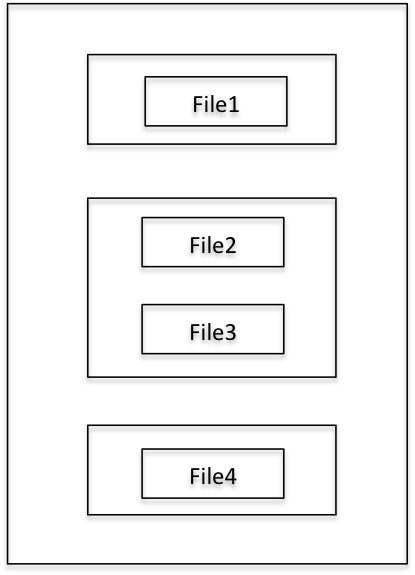
\includegraphics[scale=0.5]{figures/Containments}
%\caption{Structure of the project.}
%\label{fig:Containments}
%\end{figure}


%As described in Section \ref{} the first step of the approach is the generation of file process considering story mining techniques. Based on the comments presented in Table \ref{} the process for all four files were generated. Next the method to extract dependencies between files is run. For that the time series with the amount of change for each file is generated. Considering the correlation between the files the dependencies are found. Figure \ref{} depicts the proposed visualization of the 3 perspectives of a file.
%
%%\onecolumn{
%\begin{figure*}[t]
%\centering
%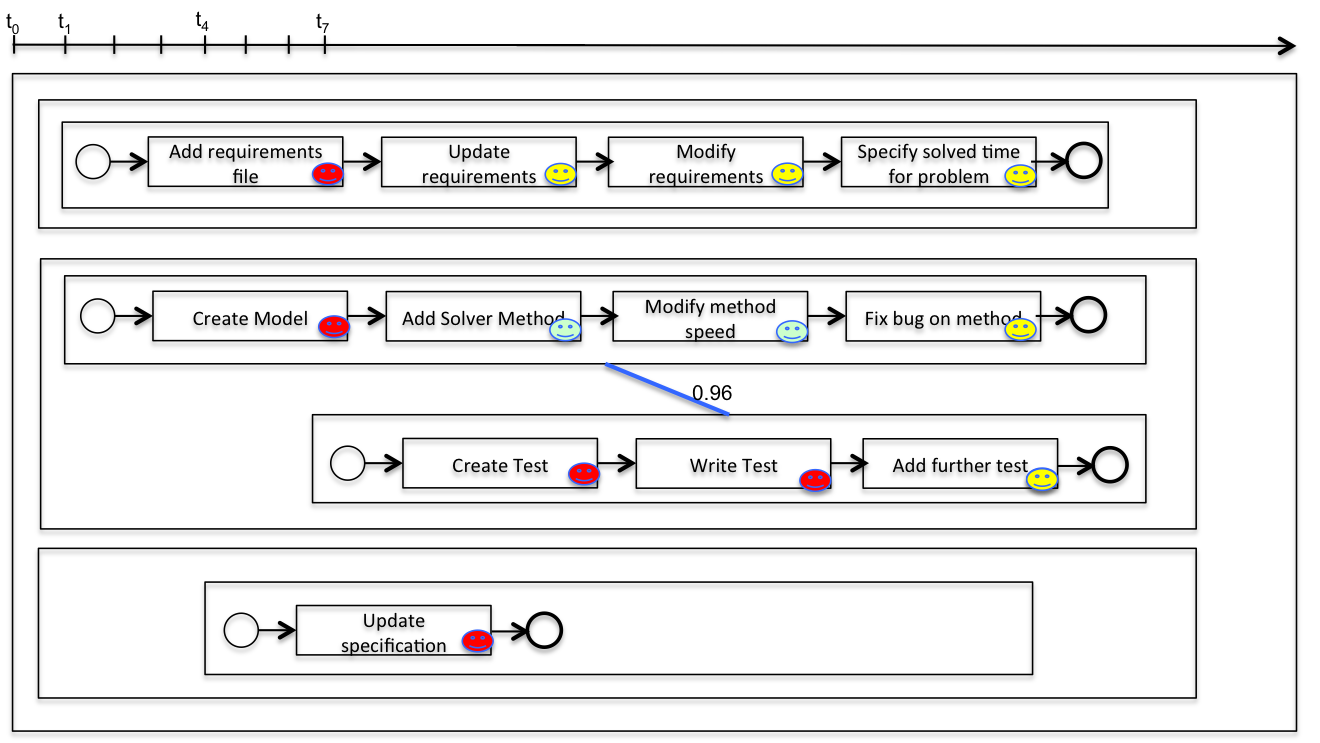
\includegraphics[scale=0.8]{figures/ExampleProposedVisualization}
%\caption{Illustration of the proposed visualization.}
%\label{fig:Containments}
%\end{figure*}
%%}

%ToDo
%Figure with the containments
%Table with the commits (junction of the .xls files. Consider only the amount of change. Express time by $t_i$
%Figure with the containments instanciated with the file processes and the dependencies.
